\documentclass[border=10pt]{standalone}
\usepackage{pgfplots}
\usepgfplotslibrary{colormaps}
\pgfplotsset{trig format plots=rad}
\begin{document}
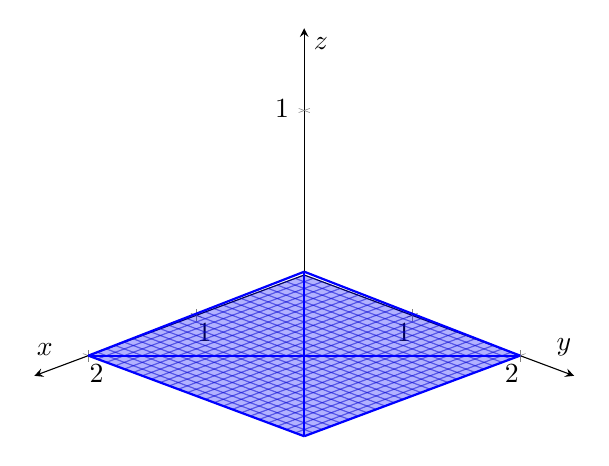
\begin{tikzpicture}
\begin{axis}[
    view={135}{30},
    xlabel=$x$, ylabel=$y$, zlabel=$z$,
    xmin=0, xmax=2.5,
    ymin=0, ymax=2.5,
    zmin=0, zmax=1.5,
    grid=major,
    axis lines=center,
]
% Let's use a more robust way to draw faces using addplot3
% Face 1: x=2 (V1, V2, V3) -> (2,2,0), (2,2,1), (2,0,0)
\addplot3[surf, opacity=0.3, domain=0:2, y domain=0:2] {0}; % This is just a placeholder
% Better: Use coordinates and simple lines to define the skeleton or use patches if they work.
% Actually, let's just draw the edges to make it clear.
% Edges:
% V1-V2: (2,2,0) to (2,2,1)
% V1-V3: (2,2,0) to (2,0,0)
% V1-V4: (2,2,0) to (0,2,0)
% V2-V3: (2,2,1) to (2,0,0)
% V2-V4: (2,2,1) to (0,2,0)
% V3-V4: (2,0,0) to (0,2,0)

\addplot3[blue, thick] coordinates {(2,2,0) (2,2,1)};
\addplot3[blue, thick] coordinates {(2,2,0) (2,0,0)};
\addplot3[blue, thick] coordinates {(2,2,0) (0,2,0)};
\addplot3[blue, thick] coordinates {(2,2,1) (2,0,0)};
\addplot3[blue, thick] coordinates {(2,2,1) (0,2,0)};
\addplot3[blue, thick] coordinates {(2,0,0) (0,2,0)};

\end{axis}
\end{tikzpicture}
\end{document}
